\documentclass{article}

\usepackage[polish]{babel}
\usepackage{polski}
\usepackage[utf8]{inputenc}

\usepackage{indentfirst}

\usepackage{longtable}

\usepackage{float}

\usepackage[a4paper,top=2cm,bottom=2cm,left=3cm,right=3cm,marginparwidth=1.75cm]{geometry}

\usepackage{listings}

\usepackage{pdfpages}


\usepackage{amsmath}
\usepackage{graphicx}
\usepackage{csquotes}
\MakeOuterQuote{"}
% \usepackage[colorlinks=true, allcolors=blue]{hyperref}

\lstdefinelanguage{AMPL}{keywords={set,param,var,arc,integer,minimize,maximize,subject,to,node,sum,in,Current,complements,integer,solve_result_num,IN,contains,less,suffix,INOUT,default,logical,sum,Infinity,dimen,max,symbolic
,Initial,div,min,table,LOCAL,else,option,then,OUT,environ,setof ,union,all,exists,shell_exitcodeuntil,binary,forall,solve_exitcodewhile ,by,if,solve_messagewithin,check,in,solve_result
},sensitive=true,comment=[l]{\#}}

\lstset{frame=tb,
  language=AMPL,
  aboveskip=3mm,
  belowskip=3mm,
  showstringspaces=false,
  columns=flexible,
  basicstyle={\ttfamily},
  numbers=none,
  numberstyle=\tiny\color{gray},
  keywordstyle=\bfseries,
  commentstyle=\textit,
  stringstyle=\color{mauve},
  breaklines=true,
  breakatwhitespace=true,
  tabsize=3
}

\title{Raport z Projektu WSYZ}
\author{
  Wojciech Kołodziejak\\
  \and
  Mateusz Maj\\
  \and
  Aleksandra Majewska\\
  \and
  Bartłomiej Rasztabiga
}

\begin{document}
\maketitle

\section{Treść zadania}

Rozważana jest produkcja i dystrybucja podstawowych warzyw, tj. ziemniaków, kapusty, buraków i marchwi w Warszawie i okolicach.
Istnieją trzy rodzaje przedsiębiorstw:
\begin{itemize}
  \item Grupa 6 produducentów: P1...P6. Każdy z producentów produkuje każdy rodzaj warzyw jednak w różnych maksymalnych ilościach rocznych. Lokalizacja producentów to: Błonie, Książenice, Góra Kalwaria, Otwock, Wołomin, Legionowo.
  \item Sieć 3 magazynów-chłodni: M1..M3. Każdy magazyn ma określoną pojemność wyrażoną w tonach (800, 1200, 750) i może służyć do przechowywania dowolnych warzyw. Lokalizacje magazynów to Pruszków, Piaseczno, Zielonka.
  \item Sieć sklepów spożywczych usytuowanych w Warszawie.
\end{itemize}

\begin{center}
\begin{longtable}{|c c|} 
\caption{Producenci} \\
\hline
nazwa & adres \\
\hline \hline
P1 & Błonie \\
\hline P2 & Książenice \\
\hline P3 & Góra Kalwaria \\
\hline P4 & Otwock \\
\hline P5 & Wołomin \\
\hline P6 & Legionowo \\
\hline
\end{longtable}
\end{center}

\begin{center}
\begin{longtable}{|c c|} 
\caption{Magazyny} \\
\hline
nazwa & adres \\
\hline \hline
M1 & Pruszków \\
\hline M2 & Piaseczno \\
\hline M3 & Zielonka \\
\hline
\end{longtable}
\end{center}

\begin{center}
\begin{longtable}{|c c c c|} 
\caption{Sklepy} \\
\hline
nazwa & adres & współrzędne & pojemność magazynu \\
\hline \hline
S1 & Béli Bartóka 8, 02-787 Warszawa & (52.162260, 21.028860) & 7,10 t \\
\hline S2 & Sady Żoliborskie 2, 01-772 Warszawa & (52.267020, 20.974340) & 7,18 t \\
\hline S3 & al. Jerozolimskie 184, 02-486 Warszawa & (52.200650, 20.932470) & 7,19 t \\
\hline S4 & Sportowa 30, 05-090 Raszyn & (52.150160, 20.930130) & 7,22 t \\
\hline S5 & Jana Pawła Woronicza 17, 00-999 Warszawa & (52.188710, 21.011170) & 7,18 t \\
\hline S6 & Aleksandra Gierymskiego 19, 00-772 Warszawa & (52.200830, 21.034420) & 7,23 t \\
\hline S7 & Jana Nowaka-Jeziorańskiego 44/U1, 03-982 Warszawa & (52.230050, 21.078680) & 7,29 t \\
\hline S8 & plac Stanisława Małachowskiego 2, 00-066 Warszawa & (52.238890, 21.012850) & 7,18 t \\
\hline S9 & Jana Ciszewskiego 15, 02-777 Warszawa & (52.153782, 21.039921) & 7,21 t \\
\hline S10 & Górczewska 88, 01-117 Warszawa & (52.239310, 20.945250) & 7,23 t \\
\hline
\end{longtable}
\end{center}

Na mapie oznaczono kolejno {\color{blue} producentów}, {\color{violet} magazyny} i {\color{red} sklepy}

\begin{figure}[H]
\centering
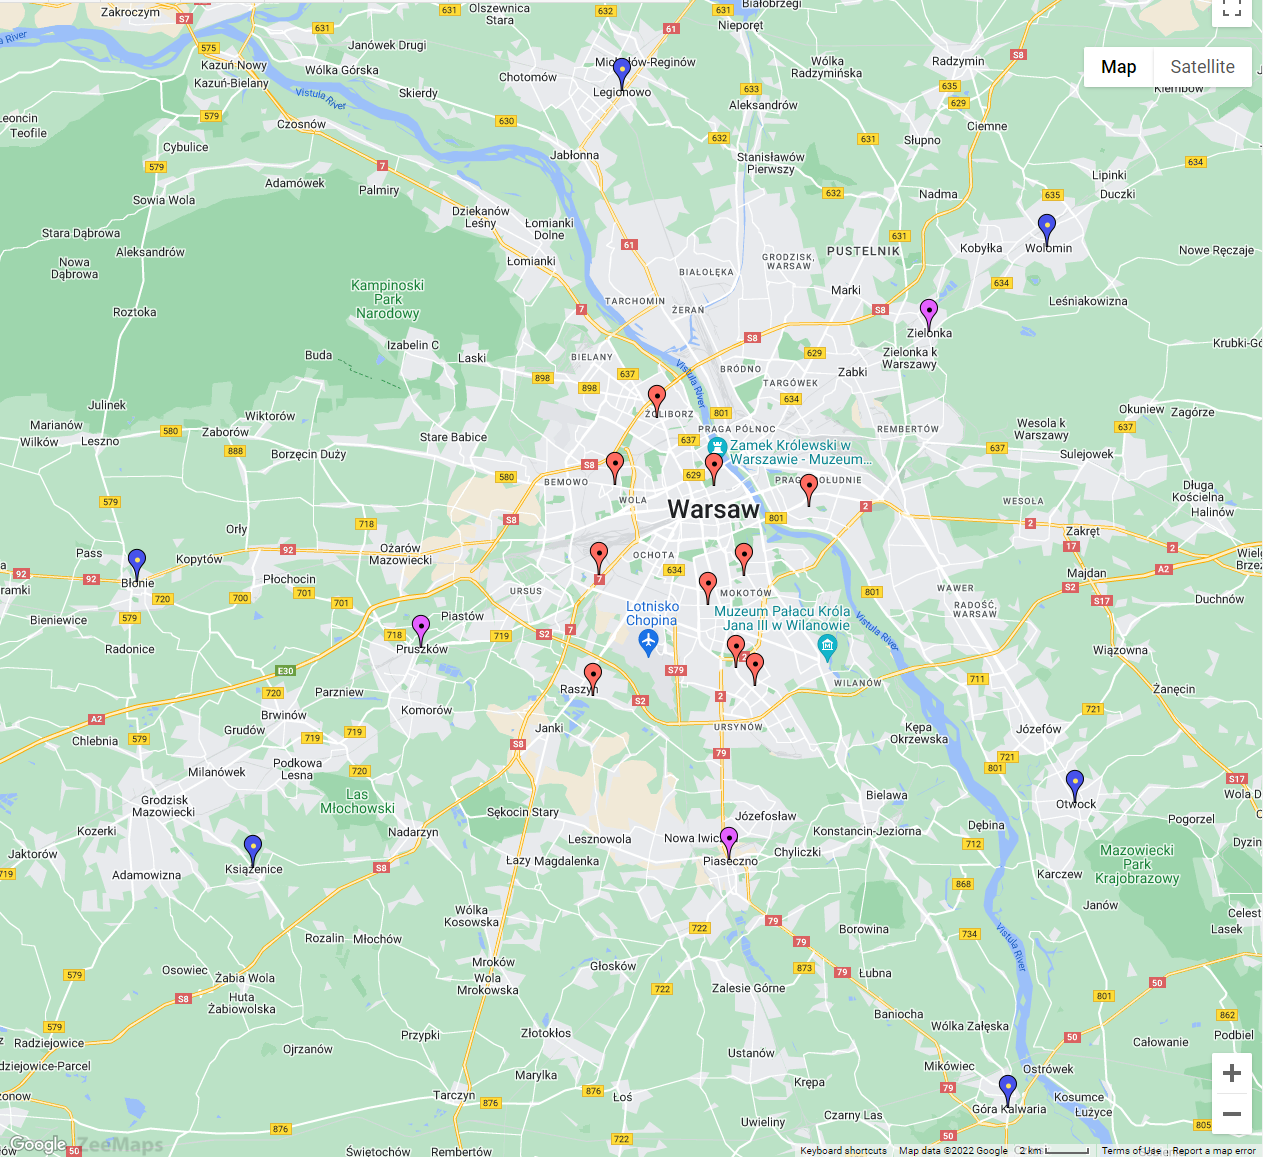
\includegraphics[scale=0.5]{map.png}
\end{figure}

\section{Model biznesowy}

Model biznesowy w notacji BPMN został zaprojektowany w aplikacji Bizagi Modeler.

// TODO opis modelu i kolejnych sekcji

\begin{figure}[H]
\caption{BPMN 1}
\centering
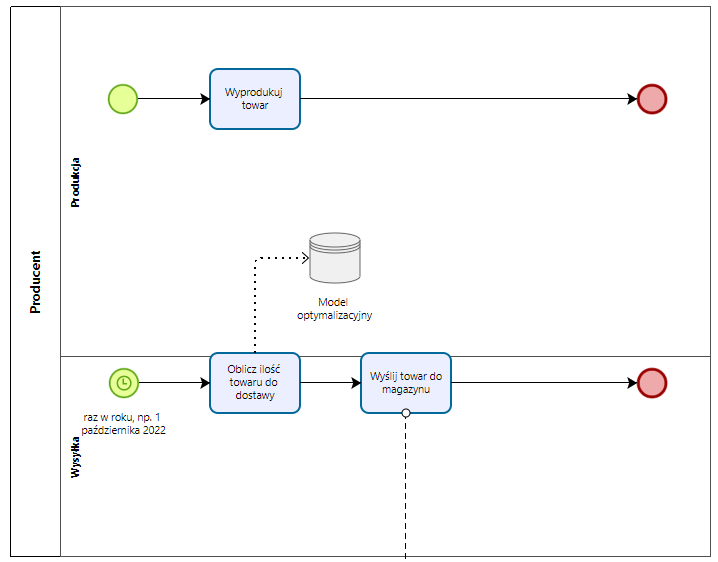
\includegraphics[scale=0.7]{bpmn1.png}
\end{figure}

\begin{figure}[H]
\caption{BPMN 2}
\centering
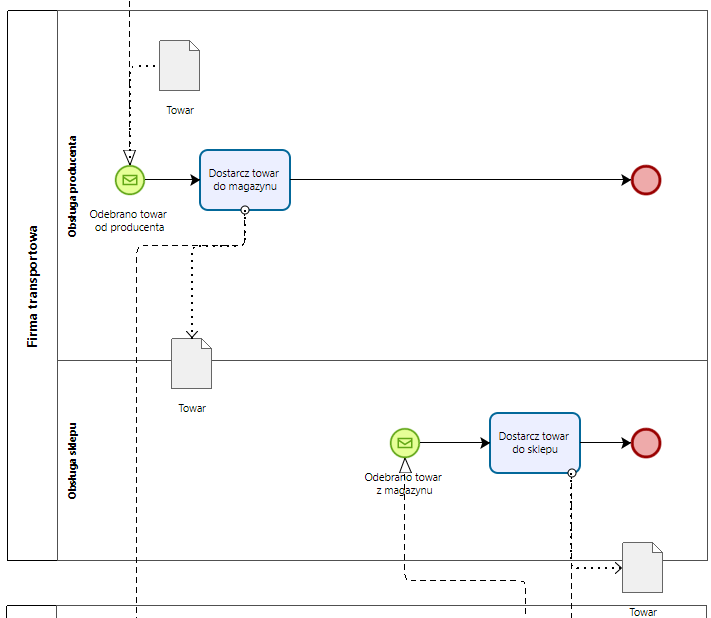
\includegraphics[scale=0.7]{bpmn2.png}
\end{figure}

\begin{figure}[H]
\caption{BPMN 3}
\centering
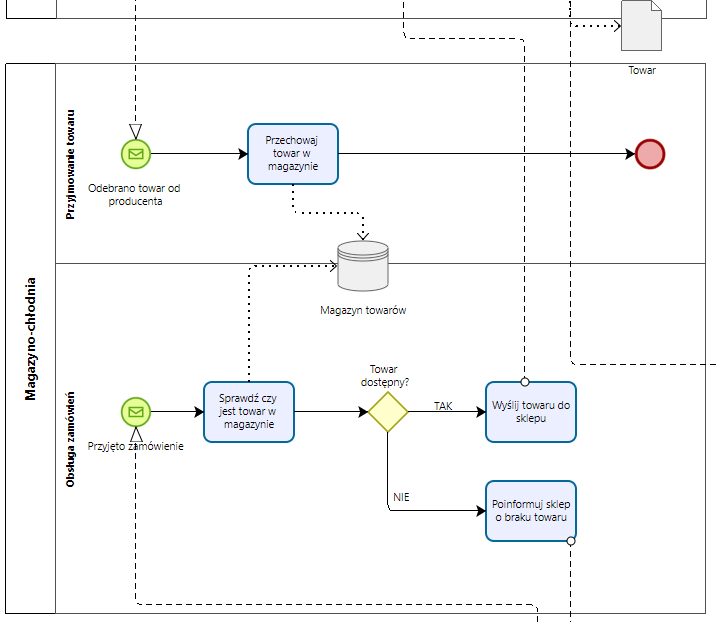
\includegraphics[scale=0.7]{bpmn3.png}
\end{figure}

\begin{figure}[H]
\caption{BPMN 4}
\centering
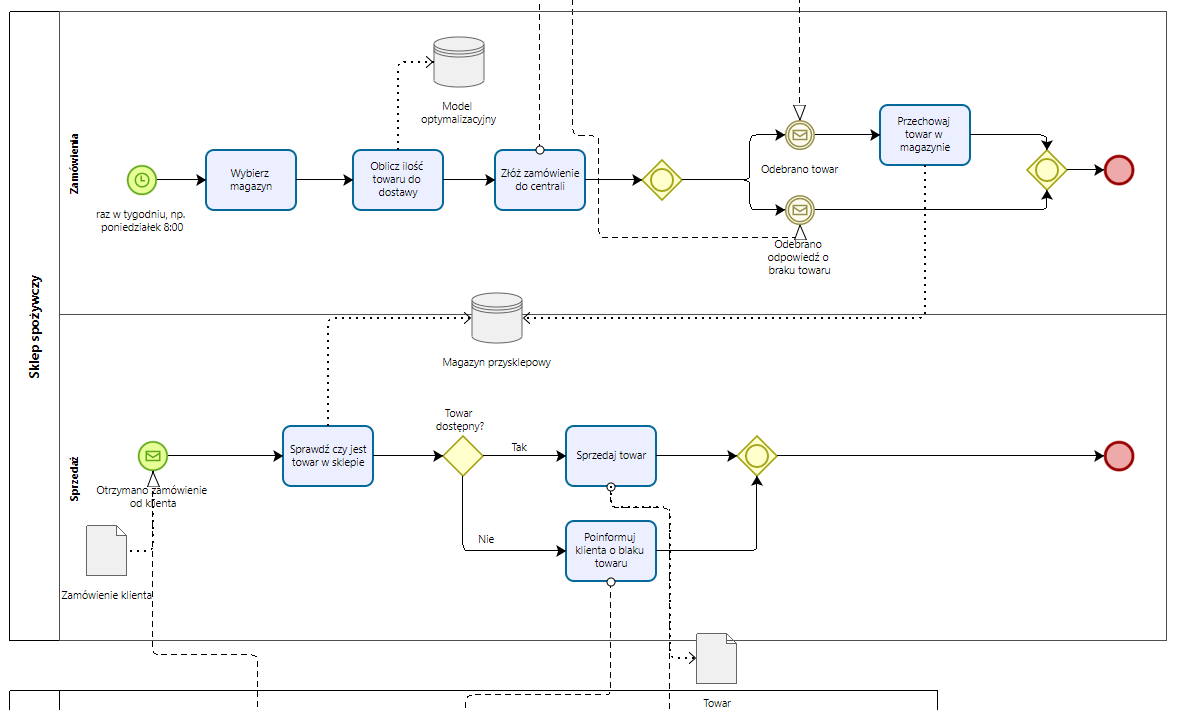
\includegraphics[scale=0.48]{bpmn4.png}
\end{figure}

\begin{figure}[H]
\caption{BPMN 5}
\centering
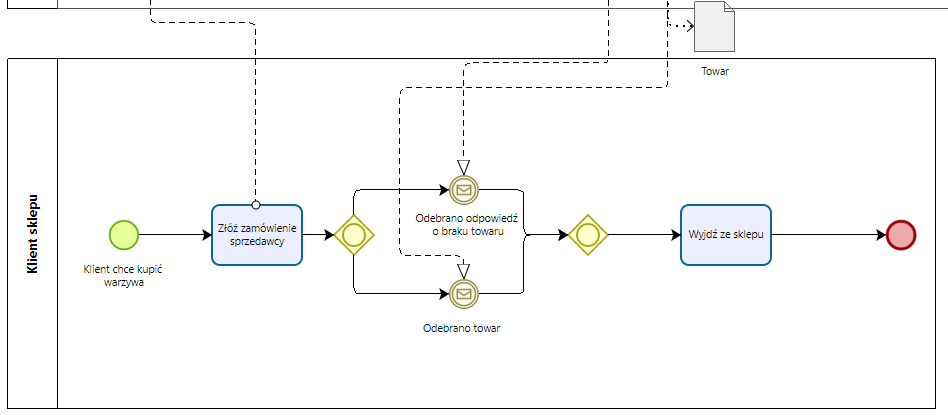
\includegraphics[scale=0.58]{bpmn5.png}
\end{figure}




\section{Model optymalizacyjny}

\subsection{Opis modelu}

Nasz model składa się z:

\begin{itemize}
   \item 4 zbiorów
   \item 8 parametrów
   \item 3 zmiennych decyzyjnych
   \item 7 ograniczeń
   \item funkcji celu
 \end{itemize}
 
Zbiory:
\begin{itemize}
   \item producenci (P1 - P6)
   \item magazyny (M1 - M3)
   \item warzywa (ziemniaki, kapusta, buraki, marchew)
   \item sklepy (S1 - S10)
 \end{itemize}
 
Parametry:
\begin{itemize}
   \item tygodnie w roku (52)
   \item podaż producentów
   \item maksymalna pojemność magazynów
   \item odległości od producentów do magazynów
   \item odległości od magazynów do sklepów
   \item prognozowana sprzedaż warzyw (dla każego tygodnia)
   \item maksymalna pojemność przysklepowych magazynów
   \item koszt transportu 1 tony na odległość 1 kilometra
 \end{itemize}
 
  
Zmienne decyzyjne:
\begin{itemize}
   \item coroczny transport od producentów do magazynów (ile producenci muszą wyprodukować)
   \item cotygodniowy transport od magazynów do sklepów
   \item cptygodniowy stan zapasu warzyw w magazynach przysklepowych
 \end{itemize}
 
Ograniczenia:
\begin{itemize}
   \item stan zapasu warzyw w sklepie jest z tygodnia na tydzień zmniejszany o prognozę sprzedaży i zwiększany o cotygodniowy transport do sklepu
   \item zapas warzyw w sklepie nie może przekroczyć maksymalnej pojemności przysklepowego magazynu
   \item cotygodniowy transport warzyw nie może przekroczyć maksymalnej pojemności przysklepowego magazynu
   \item minimalny zapas warzyw sklepie musi minimalnie wynosić 10\% prognozy sprzedaży
   \item coroczny transport do magazynów musi być większy lub równy od transportu do sklepów
   \item coroczny transport do magazynów musi być mniejszy lub równy podaży producentów
   \item coroczny transport do magazynów musi być mniejszy lub równy maksymalnej pojemności magazynów
 \end{itemize}

\subsection{Zapis modelu w AMPL}

\begin{lstlisting}
set PRODUCENTS;
set WAREHOUSES;
set VEGETABLES;
set STORES;

param T > 0;
param supply 					{PRODUCENTS,VEGETABLES} > 0;
param max_warehouse_capacity 	{WAREHOUSES} >= 0;
param distance_to_warehouse 	{PRODUCENTS,WAREHOUSES} > 0;
param distance_to_store 		{WAREHOUSES,STORES} > 0;
param weekly_sales_forecast 	{1..T, STORES, VEGETABLES} >= 0;
param store_warehouse_capacity 	{STORES} >= 0;
param km_cost > 0;

var yearly_transport_to_warehouses {PRODUCENTS,WAREHOUSES,VEGETABLES} >= 0;
var weekly_transport_to_stores {1..T,WAREHOUSES,STORES,VEGETABLES} >= 0;
var weekly_stores_warehouse_stock {1..T,STORES,VEGETABLES} >= 0;

minimize Total_Cost:
	sum {p in PRODUCENTS, w in WAREHOUSES, v in VEGETABLES}
   		distance_to_warehouse[p,w] * km_cost * yearly_transport_to_warehouses[p,w,v]
	+
	sum {w in WAREHOUSES, s in STORES, v in VEGETABLES, n in 1..T}
   		distance_to_store[w,s] * km_cost *  weekly_transport_to_stores[n,w,s,v];
    
subject to Store_Warehouse_Demand {s in STORES, n in 2..T, v in VEGETABLES}:
	weekly_stores_warehouse_stock[n, s, v] = weekly_stores_warehouse_stock[n-1, s, v] - weekly_sales_forecast[n, s, v] + sum {w in WAREHOUSES} weekly_transport_to_stores[n, w, s, v];
	
subject to Store_Warehouse_Demand_1_week {s in STORES, v in VEGETABLES}:
	weekly_stores_warehouse_stock[1, s, v] = - weekly_sales_forecast[1, s, v] + sum {w in WAREHOUSES} weekly_transport_to_stores[1, w, s, v];

subject to Store_Warehouse_Max_Capacity {s in STORES, n in 1..T}:
	sum {v in VEGETABLES} weekly_stores_warehouse_stock[n, s, v] <= store_warehouse_capacity[s];
	
subject to Store_Warehouse_Min_Capacity {s in STORES, n in 1..T, v in VEGETABLES}:
	weekly_stores_warehouse_stock[n, s, v] >= 0.1 * weekly_sales_forecast[n, s, v];
	
subject to Store_Warehouse_Max_Capacity_Transport {s in STORES, n in 1..T}:
	sum {w in WAREHOUSES, v in VEGETABLES} weekly_transport_to_stores[n, w, s, v] <= store_warehouse_capacity[s];
	
subject to Warehouse_Supply {w in WAREHOUSES, v in VEGETABLES}:
	sum {p in PRODUCENTS} yearly_transport_to_warehouses[p, w, v] >= sum {s in STORES, n in 1..T} weekly_transport_to_stores[n, w, s, v];

subject to Producent_Supply {p in PRODUCENTS, v in VEGETABLES}:
	sum {w in WAREHOUSES} yearly_transport_to_warehouses[p,w,v] <= supply[p, v];

subject to Warehouse_Max_Capacity {w in WAREHOUSES}:
	sum {p in PRODUCENTS, v in VEGETABLES} yearly_transport_to_warehouses[p,w,v] <= max_warehouse_capacity[w];
\end{lstlisting}

\section{Wyniki i wnioski}

Dla ustalonych danych wejściowych (transp.dat) całkowity minimalny koszt transportu wyniósł: 248 837 zł.

Minimalna suma pojemności magazynów do rozwiązania problemu wynosi 1881 ton. Poniżej tej wartości nie da się znaleźć rozwiązania dla zadanego popytu (prognozy sprzedaży). Oryginalnie (z treści zadania) wynosiła ona 2750 ton.

Poniżej wyniki symulacji (koszt transportu), jeżeli cały towar byłby transportowany do/z tylko jednego magazynu. 

\begin{figure}[H]
\centering
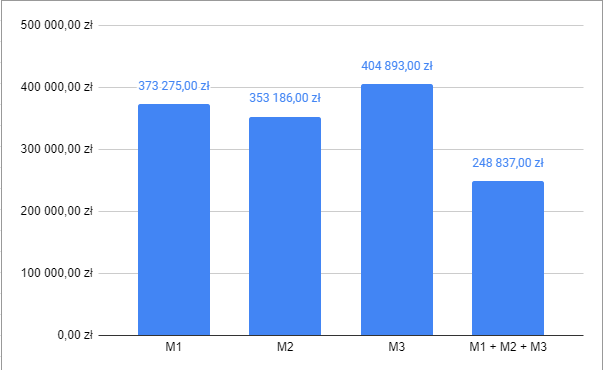
\includegraphics[scale=0.7]{wykres1.png}
\end{figure}

Jak widać, rozkład transportu na różne magazyny ma sens. Koszt jest wtedy minimalny, ponieważ sklepy pobierają towar z magazynu znajdującego się najbliżej.

Analizując wynik optymalizacji (konkretnie zmienną "weekly transport to stores") można zauważyć, że niektóre magazyny w ogóle nie zaopatrują niektórych sklepów (np. M1 nie zaopatruje w buraku S5, S6, S7 i S9). Jest to spowodowane ich dużą wzajemną odległością, czyli dużym kosztem transportu.

\begin{figure}[H]
\centering
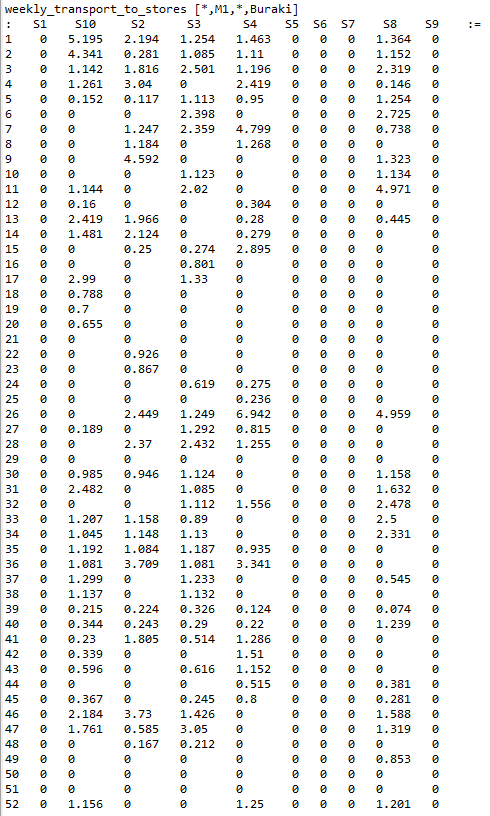
\includegraphics[scale=0.7]{ampl1.png}
\end{figure}

// TODO analiza wyniku, co by sie zmienilo, wplyw parametrow na wynik etc.

// TODO wrzucic jakies fajne wykresy (np. zaleznosc kosztu od jakiegos parametru)

\section{Harmonogram prac}

// TODO dodać osoby?

\begin{itemize}
   \item Zapoznanie się z problemem (31.03-3.04)
   \item Utworzenie modelu BPMN (3.04-6.04)
   \item Recenzja i poprawki do modelu BPMN (6.04-8.04)
   \item Ustalenie danych wejściowych do modelu optymalizacyjnego: lokalizacje sklepów (15.04-22.04)
   \item Uszczegółowienie danych wejściowych do modelu optymalizacyjnego: prognoza sprzedaży, maksymalne pojemności magazynów itd. (22.04-29.04)
   \item Utworzenie modelu optymalizacyjnego w języku AMPL (29.04-6.05)
   \item Testy rozwiązania przed oddaniem etapu (6.05-13.05)
   \item Poprawki do modelu optymalizacyjnego, dodano między innymi śledzenie stanu magazynów przysklepowych (20.05-27.05)
   \item Finalne testy rozwiązania (27.05-3.06)
   \item Utworzenie raportu z projektu (3.06-13.06)
 \end{itemize}

\end{document}